% The methodology for this research was structured as a multi-phase experimental pipeline designed to diagnose, address, and evaluate compositional reasoning deficits in state-of-the-art diffusion models. The following sections detail the iterative process of model selection, prompt engineering, architectural modification, and multi-modal evaluation.

% \subsection{Model Selection and Baseline Configuration}
% The study began with an extensive benchmarking phase to identify a robust foundation for compositional analysis. After evaluating several iterations of the Stable Diffusion family, Stable Diffusion 3.5 (SD3.5) Large Turbo \footnote{https://huggingface.co/stabilityai/stable-diffusion-3.5-large-turbo/blob/main/LICENSE.md} was selected due to its sophisticated triple-text-encoder architecture and high-fidelity ``Turbo'' distillation.

% \subsubsection{Deterministic Controls}
% To ensure experimental reproducibility and eliminate stochastic variance during comparative analysis, all image generations were locked to a fixed seed of 42.

% \subsubsection{Hyperparameter Settings}
% Generations utilized a guidance scale \citep{zhan2026understanding} of 4.0 and 28 inference steps, adhering to the optimized defaults for the SD3.5 Turbo pipeline.

% \subsubsection{Output Format}
% Generated images were stored as raw PyTorch tensors (float32) and normalized to ensure compatibility with downstream Vision-Language Model (VLM) assessment.


% \subsection{Exploratory Pilot and Problem Identification}
% Before formalizing the dataset, an unconstrained exploratory phase was conducted to map the failure modes of the baseline SD3.5 model.

% \begin{enumerate}
%     \item Baseline Diagnostics: Initial trials confirmed that while the model achieved high photorealism, it suffered from obvious compositional failures, most notably in numerical reasoning (counting) \citep{li2025countdiffusiontexttoimagesynthesistrainingfree}, \citep{zhao2025demystifyingnumerositydiffusionmodels} and with phrase ``not'' \citep{ban2024understandingimpactnegativeprompts}. 
%     \item Spatial Blind Spots: Systematic testing revealed ``blind spots'' in basic vertical and horizontal stratification. For instance, prompts requiring objects to be ``above'' or ``to the left of'' one another frequently resulted in inverted or side-by-side placements.
%     \item Relational Complexity: We identified that SD3.5 struggled significantly with ``without'' and physical interactions (e.g., ``holding''), where objects were often merged or rendered in isolation.
% \end{enumerate}


% \subsection{Dataset Construction: Self-Bench and Standardized Prompting}
% To isolate the linguistic understanding of the text encoder from the generative capacity of the diffusion transformer, we utilized the Self-Bench \citep{jeong2025diffusionclassifiersunderstandcompositionality} framework.

% \begin{enumerate}
%     \item Class Extraction: We extracted 100 simple object classes (e.g., ``giraffe'', ``book'', ``broccoli'') to ensure that any failure in the final image could be attributed to a misunderstanding of the spatial relationship rather than the inability to render the objects themselves.
%     \item Prompt Taxonomy: A benchmark of $1,600+$ unique prompts was constructed across 13 core spatial and relational phrases: above, below, to the left of, to the right of, between, behind, closeby, far from, in front of, on top of, under, over, and without.
%     \item Template Structure: Every prompt followed a rigid template: ``a photo of a [class1] [phrase] a [class2]'' and for ``between'', we used the prompt ``a photo of a [class1] between [class2]s''. This standardization allowed for a controlled comparison across baseline and custom model variants. 
% \end{enumerate}


% \subsection{Architectural Intervention: Encoder Replacement Pipeline}
% The central hypothesis of this work is that the primary CLIP-L text encoder (Text Encoder 1) could improve understanding of spatial semantics. We implemented a modular replacement of this component using the CLIC (Compositional Language-Image Contrastive) variants as depicted in \cref{fig:replacement}.

% \begin{figure}[ht]
% \vskip 0.2in
% \begin{center}
% \centerline{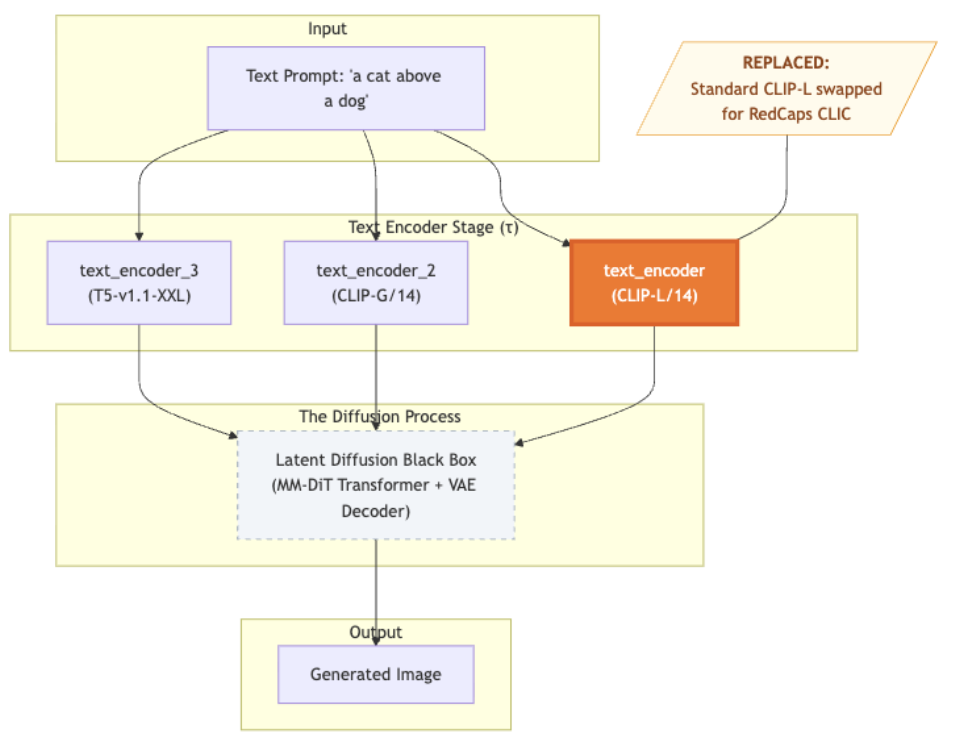
\includegraphics[width=\columnwidth]{plots/replacement.png}}
% \caption{Architectural overview of CLIP-L replacement with CLIC.}
% \label{fig:replacement}
% \end{center}
% \vskip -0.2in
% \end{figure}

% \subsubsection{CLIC Variants: RedCaps and CogVLM}
% We integrated two distinct text encoders optimized for compositional awareness:

% \begin{enumerate}
%     \item RedCaps CLIC: Trained on 12M image-text pairs from Reddit, where alt-text is frequently descriptive of spatial arrangements for accessibility.
%     \item CogVLM CLIC: A variant aligned with the CogVLM visual feature space, designed to enhance the bridge between generative modeling and discriminative spatial understanding.
% \end{enumerate}


% \subsubsection{Technical ``Weight Surgery''}
% Because the CLIC weights were distributed in the OpenCLIP format, they were architecturally incompatible with the HuggingFace-based SD3.5 pipeline. We developed a conversion utility to perform the following transformations:

% \begin{enumerate}
%     \item QKV Matrix Decomposition: The fused in\_proj\_weight $[2304, 768]$ was split into three separate $Q, K,$ and $V$ projections each of $[768, 768]$.
%     \item Activation Alignment: The configuration was explicitly set to QuickGELU ($x \cdot \text{sigmoid}(1.702 \cdot x)$). We observed that failure to use QuickGELU led to immediate latent distribution collapse.
%     \item Dimension and Layer Mapping: Weights were mapped from OpenCLIP's ``resblocks'' to HuggingFace's ``encoder.layers'' format, including a transpose operation on the final text\_projection matrix.
% \end{enumerate}

% \subsubsection{Token Length}
% The CLIPTokenizer is padded or capped with a max token length of 77 to fit the standard SD architecture requirement.


% \subsection{Multi-Prompt Evaluation}
% To analyze the resulting 3,000+ images we tried LLaVa \citep{liu2023visualinstructiontuning} and Qwen3-VL. QWEN outputs matched more with the manual annotation as compared to LLaVa \citep{chen2025why} across a subset of phrases: ``above'', ``below'', ``to the left of'', ``to the right of'' and ``between''. Hence, we utilized the Qwen3-VL-30B-A3B-Instruct model \footnote{https://huggingface.co/Qwen/Qwen3-VL-30B-A3B-Instruct}. To ensure robust assessment, we employed three distinct prompting strategies \citep{liu2023designguidelinespromptengineering} for the evaluator:
% \begin{enumerate}
%     \item Direct Query: A simple binary question regarding the spatial relationship as ``Is the {class1} {phrase} the {class2}? Answer Yes, No, or Ambiguous.''

%     \item Context-Prime (Expert Role): Using a system prompt with context \citep{zhang2024multimodalchainofthoughtreasoninglanguage}: ``You are an Expert Visual Analyst and expert at spatial reasoning. 1. Identify the {class1} and describe its position. 2. Identify the {class2} and describe its position. 3. Based on their relative coordinates, is the {class1} {phrase} the {class2}? Conclusion: [Yes/No/Ambiguous]''. This mode generated reasoning traces that provided insight into VLM failure modes. For ``between'', we used ``You are an expert at spatial reasoning. Task: Is the {class1} between the {class2}? Step 1: Identify and locate the {class1}. Step 2: Identify the group of {class2} or the boundary objects. Step 3: Analyze if the {class1} is positioned in the intermediate space separating the {class2}. Conclusion: [Yes/No/Ambiguous]''.

%     \item Inverse Logic: Prompting the VLM to describe the relationship present in the image to cross-reference against the original generative prompt. We used the prompt ``You are an Expert Visual Analyst and expert at spatial reasoning. 1. Is the {class2} {inverse\_phrase} the {class1}? 2. If so, then the {class1} is {phrase} the {class2}. Conclusion: [Yes/No/Ambiguous]''.
% \end{enumerate}


% \subsection{Manual Annotation and Fidelity Benchmarking}
% To ground the automated metrics, a comprehensive manual validation was conducted. This included the following:

% \begin{enumerate}
%     \item Sampling Strategy: For each phrase and model combination, a subset of 10 to 20 images was sampled for manual review.
%     \item Labeling Scheme: Classified images into three categories: Correct, Incorrect, or Ambiguous. This allowed for the calculation of inter-evaluator agreement with the Qwen3-VL predictions.
%     \item FID Calculation: General image fidelity was measured using FID. We generated 1,000 images per model variant using COCO \citep{lin2015microsoftcococommonobjects} validation captions and compared these distributions against the ground-truth COCO validation set to ensure no degradation in visual quality occurred during the encoder replacement.
% \end{enumerate}


% \subsection{Hardware and Computational Environment}
% Experiments were executed on University of Tübingen high-performance cluster utilizing NVIDIA A100 (40GB) GPUs. The software environment was built on diffusers 0.24.0 and transformers 4.35.0. The total computational cost, including exploratory pilots, weight conversion, large-scale generation, and VLM inference, totaled approximately 150 GPU hours.


The methodology for this research was structured as a multi-phase experimental pipeline designed to diagnose, address, and evaluate compositional reasoning deficits in state-of-the-art diffusion models. The following sections detail the iterative process of model selection, prompt engineering, architectural modification, and multi-modal evaluation.

\subsection{Model Selection and Baseline Configuration}
The study began with an extensive benchmarking phase to identify a robust foundation for compositional analysis. After evaluating several iterations of the Stable Diffusion family, Stable Diffusion 3.5 (SD3.5) Large Turbo\footnote{\url{https://huggingface.co/stabilityai/stable-diffusion-3.5-large-turbo/blob/main/LICENSE.md}} was selected due to its sophisticated triple-text-encoder architecture and high-fidelity ``Turbo'' distillation.

\subsubsection{Deterministic Controls}
To ensure experimental reproducibility and eliminate stochastic variance during comparative analysis, all image generations were locked to a fixed random seed of 42.

\subsubsection{Hyperparameter Settings}
Generations utilized a guidance scale \citep{zhan2026understanding} of 4.0 and 28 inference steps, adhering strictly to the optimized defaults for the SD3.5 Turbo pipeline.

\subsubsection{Output Format}
Generated images were stored as raw PyTorch tensors (\texttt{float32}) and systematically normalized to ensure compatibility with downstream Vision-Language Model (VLM) assessment frameworks.

\subsection{Exploratory Pilot and Problem Identification}
Before formalizing the evaluation dataset, an unconstrained exploratory phase was conducted to map the specific failure modes of the baseline SD3.5 model.

\begin{enumerate}
    \item \textbf{Baseline Diagnostics:} Initial trials confirmed that while the model achieved exceptional photorealism, it suffered from obvious compositional failures. These were most notable in numerical reasoning (counting) \citep{li2025countdiffusiontexttoimagesynthesistrainingfree, zhao2025demystifyingnumerositydiffusionmodels} and in processing logical negations such as the phrase ``not'' \citep{ban2024understandingimpactnegativeprompts}. 
    \item \textbf{Spatial Blind Spots:} Systematic testing revealed persistent ``blind spots'' in basic vertical and horizontal stratification. For instance, prompts requiring objects to be ``above'' or ``to the left of'' one another frequently resulted in inverted coordinates or side-by-side placements.
    \item \textbf{Relational Complexity:} We identified that SD3.5 struggled significantly with exclusion (e.g., ``without'') and physical interactions (e.g., ``holding''), where objects were often inappropriately merged or rendered in complete isolation.
\end{enumerate}

\subsection{Dataset Construction: Self-Bench and Standardized Prompting}
To explicitly isolate the linguistic understanding of the text encoder from the generative capacity of the diffusion transformer, we utilized the Self-Bench \citep{jeong2025diffusionclassifiersunderstandcompositionality} framework.

\begin{enumerate}
    \item \textbf{Class Extraction:} We extracted 100 simple, visually distinct object classes (e.g., ``giraffe'', ``book'', ``broccoli'') to ensure that any failure in the final image could be confidently attributed to a misunderstanding of the spatial relationship, rather than an inability to render the objects themselves.
    \item \textbf{Prompt Taxonomy:} A comprehensive benchmark of over 1,600 unique prompts was constructed across 13 core spatial and relational phrases: above, below, to the left of, to the right of, between, behind, closeby, far from, in front of, on top of, under, over, and without.
    \item \textbf{Template Structure:} Every prompt followed a rigid syntactic template: ``a photo of a [class1] [phrase] a [class2]''. For the phrase ``between'', we adapted the template to: ``a photo of a [class1] between [class2]s''. This strict standardization allowed for controlled, apples-to-apples comparisons across the baseline and custom model variants. 
\end{enumerate}

\subsection{Architectural Intervention: Encoder Replacement Pipeline}
The central hypothesis of this work is that replacing the primary CLIP-L text encoder (Text Encoder 1) with a compositionally aware alternative can significantly improve the model's understanding of spatial semantics. We implemented a modular replacement of this component using CLIC (Compositional Language-Image Contrastive) variants, as depicted in \cref{fig:replacement}.

\begin{figure}[ht]
\vskip 0.2in
\begin{center}
\centerline{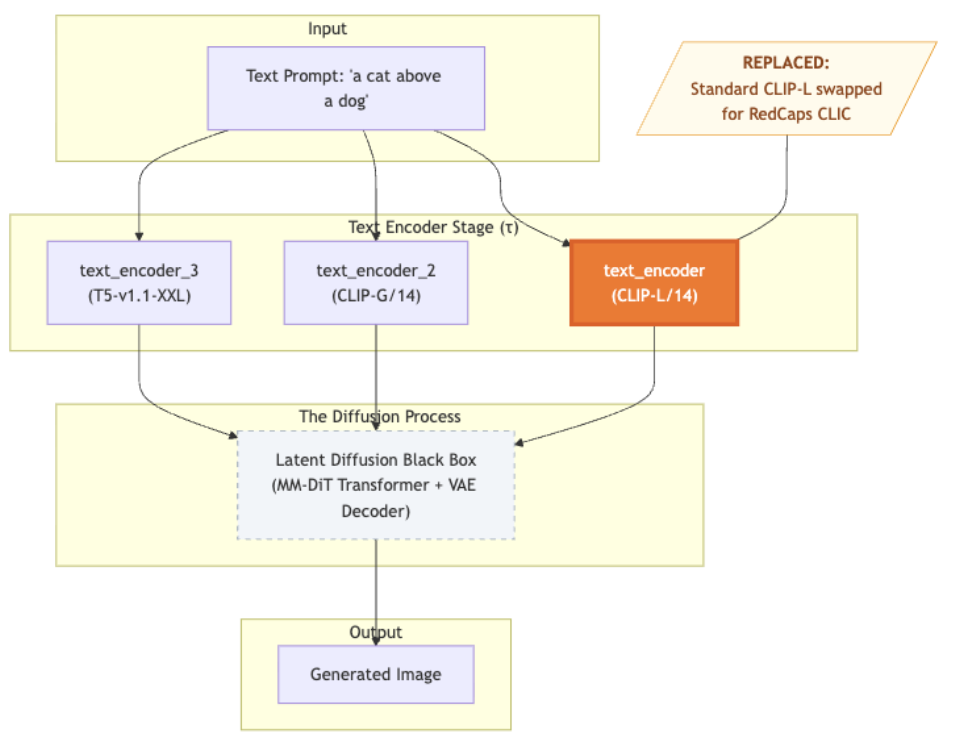
\includegraphics[width=\columnwidth]{plots/replacement.png}}
\caption{Architectural overview of the CLIP-L replacement with CLIC.}
\label{fig:replacement}
\end{center}
\vskip -0.2in
\end{figure}

\subsubsection{CLIC Variants: RedCaps and CogVLM}
We integrated two distinct text encoders inherently optimized for compositional awareness:

\begin{enumerate}
    \item \textbf{RedCaps CLIC:} Trained on 12 million image-text pairs sourced from Reddit, where alt-text frequently features highly descriptive spatial arrangements intended for accessibility.
    \item \textbf{CogVLM CLIC:} A variant aligned with the CogVLM visual feature space, specifically designed to enhance the bridge between generative modeling and discriminative spatial understanding.
\end{enumerate}

\subsubsection{Technical ``Weight Surgery''}
Because the CLIC weights were distributed in the OpenCLIP format, they were architecturally incompatible out-of-the-box with the HuggingFace-based SD3.5 pipeline. To resolve this, we developed a custom conversion utility to perform the following transformations:

\begin{enumerate}
    \item \textbf{QKV Matrix Decomposition:} The fused \texttt{in\_proj\_weight} matrix of shape $2304 \times 768$ was mathematically split into three separate Query ($Q$), Key ($K$), and Value ($V$) projections, each possessing a shape of $768 \times 768$.
    \item \textbf{Activation Alignment:} The model configuration was explicitly updated to use the QuickGELU activation function, defined as $x \cdot \text{sigmoid}(1.702 \cdot x)$. We empirically observed that failure to align with QuickGELU led to immediate latent distribution collapse during generation.
    \item \textbf{Dimension and Layer Mapping:} Weights were systematically mapped from OpenCLIP's \texttt{resblocks} nomenclature to HuggingFace's \texttt{encoder.layers} format, which included performing a necessary transpose operation on the final \texttt{text\_projection} matrix.
\end{enumerate}

\subsubsection{Token Length}
To satisfy standard Stable Diffusion architectural requirements, the \texttt{CLIPTokenizer} was strictly padded or truncated to a maximum token length of 77.

\subsection{Multi-Prompt Evaluation}
To analyze the resulting dataset of over 3,000 generated images, we initially evaluated both LLaVa \citep{liu2023visualinstructiontuning} and Qwen3-VL. Our pilot analysis revealed that Qwen3-VL outputs aligned much more closely with manual human annotations compared to LLaVa \citep{chen2025why} across a critical subset of phrases (``above'', ``below'', ``to the left of'', ``to the right of'', and ``between''). Consequently, we utilized the Qwen3-VL-30B-A3B-Instruct model\footnote{\url{https://huggingface.co/Qwen/Qwen3-VL-30B-A3B-Instruct}} for the primary evaluation. To ensure robust assessment, we employed three distinct prompting strategies \citep{liu2023designguidelinespromptengineering} for the VLM evaluator:

\begin{enumerate}
    \item \textbf{Direct Query:} A simple binary question regarding the spatial relationship, formatted as: \textit{``Is the \{class1\} \{phrase\} the \{class2\}? Answer Yes, No, or Ambiguous.''}

    \item \textbf{Context-Prime (Expert Role):} Leveraging a system prompt with established context \citep{zhang2024multimodalchainofthoughtreasoninglanguage}: \textit{``You are an Expert Visual Analyst and expert at spatial reasoning. 1. Identify the \{class1\} and describe its position. 2. Identify the \{class2\} and describe its position. 3. Based on their relative coordinates, is the \{class1\} \{phrase\} the \{class2\}? Conclusion: [Yes/No/Ambiguous].''} This multi-step mode successfully generated reasoning traces that provided deeper insights into VLM failure modes. For the phrase ``between'', the prompt was modified to: \textit{``You are an expert at spatial reasoning. Task: Is the \{class1\} between the \{class2\}s? Step 1: Identify and locate the \{class1\}. Step 2: Identify the group of \{class2\}s or the boundary objects. Step 3: Analyze if the \{class1\} is positioned in the intermediate space separating the \{class2\}s. Conclusion: [Yes/No/Ambiguous].''}

    \item \textbf{Inverse Logic:} Prompting the VLM to describe the relationship present in the image to cross-reference against the original generative prompt: \textit{``You are an Expert Visual Analyst and expert at spatial reasoning. 1. Is the \{class2\} \{inverse\_phrase\} the \{class1\}? 2. If so, then the \{class1\} is \{phrase\} the \{class2\}. Conclusion: [Yes/No/Ambiguous].''}
\end{enumerate}

\subsection{Manual Annotation and Fidelity Benchmarking}
To ground the automated metrics and ensure VLM reliability, a comprehensive manual validation was conducted, comprising the following steps:

\begin{enumerate}
    \item \textbf{Sampling Strategy:} For each phrase and model combination, a representative subset of 10 to 20 images was sampled for rigorous manual review.
    \item \textbf{Labeling Scheme:} Manual annotation classified images into three distinct categories: Correct, Incorrect, or Ambiguous. This process allowed for the calculation of inter-evaluator agreement with the automated Qwen3-VL predictions.
    \item \textbf{FID Calculation:} General image fidelity was measured using the Fréchet Inception Distance (FID) via the \texttt{pytorch-fid} library. We generated 5,000 images per model variant using standard COCO \citep{lin2015microsoftcococommonobjects} validation captions. Following standard protocols, features were extracted using a pre-trained InceptionV3 network at the 2048-dimensional pooling layer with a batch size of 50. These distributions were then compared against the ground-truth COCO validation set to ensure that no overarching degradation in visual quality occurred as a side-effect of the encoder replacement.
\end{enumerate}

\subsection{Hardware and Computational Environment}
All experiments were executed on the University of Tübingen's high-performance cluster, utilizing NVIDIA A100 (40GB) GPUs. The software environment was built utilizing \texttt{diffusers} version 0.24.0 and \texttt{transformers} version 4.35.0. The total computational footprint—including exploratory pilots, weight conversion, large-scale generation, and VLM inference—amounted to approximately 150 GPU hours.